This chapter goes into the detail about the mathematics used in the proposed framework, dealing with modeling, planning and optimization.
\section{Quadrotor Mathematical Model}
The aerial platforms chosen for the simulation are two planar quadcopters, one equipped with a camera rigidly mounted along its body $x$-axis and the other one with an end-effector on which a force sensor is mounted at the tip. 
\\The mathematical model can be considered as in common for both an it's a well-known quadcopter mathematical model. Let $m$ be the total mass of the drone, $\mathbf{g}=\begin{bmatrix}0 & 0 & g_0\end{bmatrix}^\top$ the gravity vector, and $\mathbf{J}=\operatorname{diag}(I_{xx},I_{yy},I_{zz})$ the diagonal inertia matrix. The 6-DoF rigid body dynamics can be expressed as follows:
\begin{equation} \label{eq:quadrotor_model}
\begin{aligned}
\dot{\mathbf{p}} &= \mathbf{v},\\
\dot{\mathbf{v}} &= \frac{1}{m}\,\mathbf{R}(\mathbf{q}) \begin{bmatrix}0\\[1mm]0\\[1mm]F_z\end{bmatrix} - \mathbf{g + \dfrac{1}{m} F_{ext}},\\
\dot{\mathbf{q}} &= \tfrac{1}{2}\,\boldsymbol{\Omega}(\boldsymbol{\omega})\,\mathbf{q}, \qquad 
\boldsymbol{\Omega}(\boldsymbol{\omega}) \!=\! \begin{bmatrix}
0 & -\omega_x & -\omega_y & -\omega_z\\
\omega_x & 0 & \omega_z & -\omega_y\\
\omega_y & -\omega_z & 0 & \omega_x\\
\omega_z & \omega_y & -\omega_x & 0
\end{bmatrix},\\
\dot{\boldsymbol{\omega}} &= \mathbf{J}^{-1}\!\left(\boldsymbol{\tau} - \boldsymbol{\omega} \times \mathbf{J}\boldsymbol{\omega}+\boldsymbol{\tau}_{ext}\right),
\end{aligned}
\end{equation}

where:
\begin{itemize}
    \item $\mathbf{p} \in \mathbb{R}^3$ is the position of the Center of Mass (CoM) in the world frame;
    \item $\mathbf{v} \in \mathbb{R}^3$ is the CoM linear velocity in the world frame;
    \item $\mathbf{q} = \begin{bmatrix} q_x & q_y & q_z & q_w \end{bmatrix}^\top$ is the unit quaternion representing the orientation of the body frame with respect to the world frame;
    \item $\boldsymbol{\omega} = \begin{bmatrix} \omega_x & \omega_y & \omega_z \end{bmatrix}^\top$ is the angular velocity expressed in the body frame;
    \item $\boldsymbol{\tau} = \begin{bmatrix} \tau_x & \tau_y & \tau_z \end{bmatrix}^\top$ and $F_z$ are the control torques and the total thrust generated by the propellers, respectively;
    \item $\mathbf{F_{ext}} \in \mathbb{R}^3$ and $\boldsymbol{\tau}_{ext} \in \mathbb{R}^3$ represent the unmodeled external forces and torques acting on the drone (e.g., aerodynamic drag, ground effect, wind, model mismatches), expressed in the world frame and body frame, respectively;
    \item $\mathbf{R}(\mathbf{q}) \in SO(3)$ is the rotation matrix from the body frame to the world frame, derived from the quaternion as:
    \begin{equation}
        \mathbf{R}(\mathbf{q}) = \begin{bmatrix}
        1-2(q_y^2+q_z^2) & 2(q_xq_y-q_zq_w) & 2(q_xq_z+q_yq_w)\\
        2(q_xq_y+q_zq_w) & 1-2(q_x^2+q_z^2) & 2(q_yq_z-q_xq_w)\\
        2(q_xq_z-q_yq_w) & 2(q_yq_z+q_xq_w) & 1-2(q_x^2+q_y^2)
        \end{bmatrix}
    \end{equation}
\end{itemize}

\section{Observer Drone: MPC-based Geometric \\Tracking}
The observer drone is designed to act as an active Point of View (PoV) for the human operator. This implies satisfying multiple simultaneous requirements: guaranteeing flight stability, maintaining the target drone within the camera's Field of View (FOV) at a desired mutual distance, ensuring a specific observation angle (e.g., frontal or lateral), and providing a smooth trajectory to minimize the operator's motion sickness. 

\subsection{From Optimal Control to MPC}
Handling multiple conflicting objectives and strict state-input constraints on an underactuated system naturally leads to the formulation of an Optimal Control Problem (OCP). In general terms, given a continuous-time dynamical system $\dot{\mathbf{x}} = f(\mathbf{x}(t), \mathbf{u}(t))$, optimal control seeks a control law $\mathbf{u}_{\text{opt}}(t)$ capable of minimizing a defined cost function $J(\mathbf{x}(t), \mathbf{u}(t))$ over a finite time horizon $T_f$. The standard continuous-time OCP can be written as:
\begin{equation}
\min_{\mathbf{x},\mathbf{u}} J(\mathbf{x}, \mathbf{u}) = \min_{\mathbf{x}, \mathbf{u}} \int_{t_0}^{t_0+T_f} L(\mathbf{x}(t), \mathbf{u}(t)) \, dt + \Phi(\mathbf{x}(t_0+T_f))
\end{equation}
\begin{center}
s.t.
$\begin{cases}
    \dot{\mathbf{x}} = f(\mathbf{x} , \mathbf{u})\\
    \mathbf{x}(t_0) = \mathbf{x}_{init}\\
    \mathbf{x}(t) \in \mathcal{X}, \mathbf{u}(t) \in \mathcal{U}
\end{cases}$
\end{center}
where $L(\mathbf{x,u})$ represents the stage cost over the horizon, and $\Phi(\mathbf{x}(t_0+T_f))$ represents the terminal cost. The system is subject to the continuous dynamics(eq. \ref{eq:quadrotor_model}), initial conditions, and feasible sets for states and inputs.
\\Solving a standard OCP yields an open-loop trajectory, which is inadequate for the proposed shared-control architecture. The target drone moves dynamically, and the human operator can unpredictably alter its trajectory. Therefore, an online, closed-loop planner is required. This is achieved through Model Predictive Control (MPC).
\\To transition from the continuous-time formulation to a tractable numerical problem, the system dynamics are discretized using an Explicit Runge-Kutta (ERK) integrator. The MPC algorithm solves the resulting discrete-time OCP over a receding prediction horizon of $N$ steps at each sampling time $T_s$, generating an optimal control sequence from which only the first element is applied to the plant. This process constantly updates the initial conditions based on state feedback, providing real-time tracking, robustness against model uncertainties, and the ability to incorporate the human operator's inputs.

\subsection{NMPC Problem Formulation}
\subsubsection{Nonlinear Least Square Cost Function}
In formulating the OCP, we first define the vectors of the cost terms that need to be optimized over the prediction horizon. The stage cost vector $\mathbf{y}_k$ and the terminal cost vector $\mathbf{y}_N$ are composed of the actual system states and control inputs:
\begin{align}
    \mathbf{y}_k &= \begin{bmatrix} \mathbf{p}^T, \psi, \mathbf{v}^T, \boldsymbol{\omega}^T, \dot{\mathbf{v}}^T, \dot{\boldsymbol{\omega}}^T, \ddot{\mathbf{v}}^T, \dddot{\mathbf{v}}^T, \mathbf{u}^T \end{bmatrix}^T, \\
    \mathbf{y}_N &= \begin{bmatrix} \mathbf{p}^T, \psi, \mathbf{v}^T, \boldsymbol{\omega}^T, \dot{\mathbf{v}}_{\text{hov}}^T, \dot{\boldsymbol{\omega}}_{\text{hov}}^T, \ddot{\mathbf{v}}_{\text{hov}}^T, \dddot{\mathbf{v}}_{\text{hov}}^T \end{bmatrix}^T.
\end{align}
In this formulation, $\mathbf{p}$ is the absolute Cartesian position of the drone and $\psi$ is its actual yaw angle. The vectors $\dot{\mathbf{v}}, \ddot{\mathbf{v}}, \dddot{\mathbf{v}}$ and $\dot{\boldsymbol{\omega}}$ denote linear acceleration, jerk, snap, and angular acceleration, which are penalized to minimize the operator's motion sickness.
\\To evaluate the tracking performance, these actual terms must be compared with a reference vector $\mathbf{y}_{\text{ref},k}$. As previously stated, bringing cylindrical transformations directly into the cost evaluation introduces non-linearities and variable Jacobians. To maintain a well-conditioned numerical problem, the desired cylindrical references $(r_{ref}, \beta_{ref}, z_{rel,ref})$ are mapped externally into an absolute cartesian target position $\mathbf{p}_{\text{ref}} = [x_{\text{ref}}, y_{\text{ref}}, z_{\text{ref}}]^\top$. By inverting Eq. (\ref{eq:cyl_mapping}), this external mapping is computed as:
\begin{align}
    x_{\text{ref}} &= x_{\text{obj}} + r_{ref} \cos(\beta_{ref}), \\
    y_{\text{ref}} &= y_{\text{obj}} + r_{ref} \sin(\beta_{ref}), \\
    z_{\text{ref}} &= z_{\text{obj}} + z_{rel,ref}.
\end{align}
With the position references mapped into the absolute world frame, the complete reference vector $\mathbf{y}_{\text{ref},k}$ is assembled using $\mathbf{p}_{\text{ref}}$ and the desired yaw $\psi_{ref}$. The objective of the nonlinear MPC is then formulated as a discrete-time Nonlinear Least Squares (NLS) optimization problem, which minimizes the tracking error between the cost vectors and the reference vectors over the horizon $N$:
\begin{equation}
    \min_{\mathbf{u}, \mathbf{x}} \sum_{k=0}^{N-1} \left( \|\mathbf{y}_k - \mathbf{y}_{\text{ref},k}\|_{\mathbf{W}}^2 \right) + \|\mathbf{y}_N - \mathbf{y}_{\text{ref},N}\|_{\mathbf{W}_e}^2,
\end{equation}
where $\mathbf{W}$ and $\mathbf{W}_e$ are the diagonal weight matrices for the stage and terminal costs, respectively. By decoupling the geometrical transformations from the objective function, this strategy guarantees that the positional error tracking maintains a constant identity Jacobian, thereby improving solver stability and execution speed.
\subsubsection{Weight matrices}
Given the heterogeneous quantities in the residual vector $\mathbf{y}_k$, an unscaled weight matrix leads to numerical ill-conditioning. The diagonal weight matrices $\mathbf{W} = \operatorname{blkdiag}(\mathbf{Q}, \mathbf{R})$ and $\mathbf{W}_e$ are constructed using Bryson's rule normalization~\cite{bryson1975applied}. Each diagonal element is scaled inversely proportional to the square of its maximum expected deviation:
\begin{equation}
    W_{ii} = \frac{w_i}{(\Delta y_{i, \max})^2}
\end{equation}
where $w_i$ is the relative priority weight of the specific objective and $\Delta y_{i, \max}$ is the maximum acceptable tolerance for that state. This normalization prevents higher-order physical limits from dominating the geometric framing requirements. The terminal weight matrix $\mathbf{W}_e$ follows a similar structure, lacking the input partition $\mathbf{R}$.

\subsubsection{Constraints}
A first constraint set of te OCP is given by the system dynamics:
\begin{align}
    \mathbf{x}_{k+1} &= \mathbf{f}_d(\mathbf{x}_k, \mathbf{u}_k), \\
    \mathbf{x}_0 &= \bar{\mathbf{x}}_{\text{init}},
\end{align}
where $\mathbf{f}_d$ represents the explicit Runge-Kutta discretization of the quadrotor model represented by ~\ref{eq:quadrotor_model}. Actuation and workspace limitations are enforced via hard box constraints on the control inputs $\mathbf{u}_k = [F_z, \tau_x, \tau_y, \tau_z]^\top$:
\begin{equation}
    \begin{bmatrix} 0 \\ -U_{\tau x} \\ -U_{\tau y} \\ -U_{\tau z} \end{bmatrix} \le 
    \mathbf{u}_k \le 
    \begin{bmatrix} U_F \\ U_{\tau x} \\ U_{\tau y} \\ U_{\tau z} \end{bmatrix}.
\end{equation}
While maintaining the target in the Field of View (FOV) could be treated via explicit inequality soft-constraints, the chosen approach was to handle these constraints only with haptic feedback. Therefore, visual and safety requirements are induced through the weighted and normalized tracking cost, coupled with the external Artificial Potential Fields (APF) (see \ref{section:APF}) acting on the human input. This keeps the reference fed to the MPC within the optical frustum limits, allowing the solver to focus purely on dynamically feasible and smooth trajectory generation.
\begin{figure}[htbp]
\centering
\resizebox{\textwidth}{!}{%
\begin{tikzpicture}[
    font=\sffamily\small,
    >= {Latex[length=3mm, width=2mm]},
    % Definizione colori 
    colYellow/.style={fill=yellow!20!, draw=yellow!60!black, thick},
    colHapticBg/.style={fill=black!10!, draw=gray!80!black, dashed, thick},
    colInnerGray/.style={fill=black!10!, draw=gray!80!black, thick},
    colSwitch/.style={fill=black!0, draw=white!80, thick},
    colGreen/.style={fill=green!20!olive!20!, draw=green!40!black, thick},
    colMap/.style={fill=red!20!, draw=red!80!black!, thick},
    colUavBg/.style={fill=orange!10!, draw=orange!80!black, dashed, thick},
    colNmpc/.style={fill=orange!50!, draw=orange!80!black, thick},
    colDroneBox/.style={fill=orange!22, draw=orange!80!black, thick},
    colEkf/.style={fill=cyan!55!blue!25, draw=cyan!50!black, thick},
    % Stile linee di connessione
    conn/.style={->, draw=black!80, line width=0.7pt},
    connGray/.style={->, draw=black!60, line width=0.7pt},
    % =========================================================
    % ICONA 1: Joystick / Haptic (Disegnata nativamente in TikZ)
    % =========================================================
    joystick/.pic={
        % Base inferiore
        \fill[black!65, rounded corners=1.5pt] (-0.52,-0.42) rectangle (0.52,-0.25);
        % Gradino superiore base
        \fill[black!65] (-0.32,-0.25) rectangle (0.32,-0.16);
        % Asta
        \draw[black!65, line width=2.4pt] (0,-0.16) -- (0,0.18);
        % Sfera (Pomello)
        \fill[black!65] (0,0.24) circle (0.19);
        % Riflesso bianco sulla sfera
        \draw[white, line width=1.1pt, line cap=round] (0.04,0.34) arc (65:145:0.11);
    },
    % =========================================================
    % ICONA 2: Quadrotore con Camera (Disegnata nativamente)
    % =========================================================
    quadrotor/.pic={
        \definecolor{dronebr}{RGB}{95, 50, 15}
        % Bracci e corpo centrale
        \fill[dronebr] (-0.75, 0.10) -- (-0.20, 0.10) -- (-0.12, 0.0) -- (0.12, 0.0) -- (0.20, 0.10) -- (0.75, 0.10) -- (0.75, 0.16) -- (-0.75, 0.16) -- cycle;
        \fill[dronebr, rounded corners=2pt] (-0.28, 0.02) rectangle (0.28, 0.18);
        % Motori ed eliche
        \fill[dronebr] (-0.68, 0.16) rectangle (-0.58, 0.24);
        \fill[dronebr] (0.58, 0.16) rectangle (0.68, 0.24);
        \draw[dronebr, line width=1.4pt] (-0.92, 0.24) -- (-0.34, 0.24);
        \draw[dronebr, line width=1.4pt] (0.34, 0.24) -- (0.92, 0.24);
        % Carrelli di atterraggio
        \draw[dronebr, line width=2pt, line cap=round] (-0.26, 0.04) -- (-0.38, -0.36);
        \draw[dronebr, line width=2pt, line cap=round] (0.26, 0.04) -- (0.38, -0.36);
        % Supporto e Telecamera centrale
        \draw[dronebr, line width=1.2pt] (-0.18, -0.04) -- (0, -0.12) -- (0.18, -0.04);
        \draw[dronebr, fill=orange!22, line width=1.2pt, rounded corners=1.5pt] (-0.14, -0.34) rectangle (0.14, -0.10);
        \draw[dronebr, line width=1pt] (0, -0.22) circle (0.08);
        \fill[dronebr] (0, -0.22) circle (0.04);
    }
]

    % ---------------------------------------------------------
    % 1. CONTENITORI TRATTEGGIATI DI SFONDO
    % ---------------------------------------------------------
    % Contenitore Haptic Interface
    \node[colHapticBg, minimum width=4.4cm, minimum height=5.6cm, rounded corners] (haptic_bg) at (3.6, -1.5) {};
    \node[text=black!65, align=center, rounded corners] at (3.6, -1.45) {\textbf{Haptic}\\[-2pt]\textbf{interface}};

    % Contenitore NMPC Controlled UAV
    \node[colUavBg, minimum width=5.4cm, minimum height=4.1cm] (uav_bg) at (14.7, 0.60) {};
    \node[text=orange!35!black, align=center] at (14.7, 2.00) {\textbf{NMPC Controlled}\\[-2pt]\textbf{UAV}};

    % ---------------------------------------------------------
    % 2. BLOCCHI PRINCIPALI
    % ---------------------------------------------------------
    % Colonna Sinistra: Riferimento autonomo e Operatore Umano
    \node[colYellow, minimum width=2.4cm, minimum height=1.5cm, align=center] (auto_ref) at (1.0, 2.2) {Autonomous\\cylindrical\\reference};
    
    \node[colYellow, minimum width=1.6cm, minimum height=2.4cm, align=center] (human) at (0.4, 0.0) {Human\\operator};

    % Blocchi interni a Haptic Interface
    \node[colInnerGray, minimum width=1.6cm, minimum height=1.35cm, rounded corners] (joy_box) at (2.7, 0.0) {};
    \pic at (joy_box.center) {joystick};

    \node[colInnerGray, minimum width=1.1cm, minimum height=1.15cm, font=\large, text=black!65, rounded corners] (integrator) at (4.7, 0.0) {$\dfrac{1}{s}$};

    \node[colGreen, minimum width=3.5cm, minimum height=1.85cm, align=center, text=green!25!black, rounded corners] (apf) at (3.6, -3.2) {Force feedback\\Management\\(APF)};

    % ---------------------------------------------------------
    % BLOCCO SWITCH (Selettore Riferimento Autonomo / Aptico)
    % ---------------------------------------------------------
    \node[colSwitch, minimum width=1.0cm, minimum height=1.15cm] (switch_box) at (6.85, 0.25) {};
    % Tratti interni di collegamento ai terminali
    \draw[black!75, line width=0.7pt] (6.35, 0.50) -- (6.58, 0.50);
    \draw[black!75, line width=0.7pt] (6.35, 0.00) -- (6.58, 0.00);
    \draw[black!75, line width=0.7pt] (7.12, 0.25) -- (7.35, 0.25);
    % Leva interna dello switch e freccia di commutazione
    \draw[black!80, line width=1.1pt, line cap=round] (7.10, 0.25) -- (6.62, 0.46);
    \draw[<->, >={Latex[length=1.4mm, width=1.1mm]}, black!55, line width=0.45pt] (6.72, 0.41) to[bend right=25] (6.72, 0.09);
    % Terminali (pallini bianchi)
    \filldraw[fill=white, draw=black!80, line width=0.7pt] (6.60, 0.50) circle (0.055);
    \filldraw[fill=white, draw=black!80, line width=0.7pt] (6.60, 0.00) circle (0.055);
    \filldraw[fill=white, draw=black!80, line width=0.7pt] (7.10, 0.25) circle (0.055);

    % Colonna Centrale: Blocchi di Mapping
    \node[colMap, minimum width=1.8cm, minimum height=2.4cm, align=center, rounded corners] (cyl2cart) at (10.3, 0.25) {Cylindrical\\to\\Cartesian\\mapping};

    \node[colMap, minimum width=1.8cm, minimum height=2.4cm, align=center, rounded corners] (cart2cyl) at (10.3, -3.2) {Cartesian\\to\\Cylindrical\\mapping};

    % Blocchi interni a NMPC Controlled UAV
    \node[colNmpc, minimum width=1.4cm, minimum height=2.6cm, align=center, text=orange!25!black, font=\sffamily\bfseriesm] (nmpc) at (13.2, 0.25) {NMPC};

    \node[colDroneBox, minimum width=2.1cm, minimum height=1.15cm] (drone_box) at (15.9, 0.25) {};
    \pic at (drone_box.center) {quadrotor};

    % Blocco EKF2 in basso a destra
    \node[colEkf, minimum width=2.2cm, minimum height=0.95cm, align=center, rounded corners] (ekf) at (15.9, -3.2) {EKF2};

    % ---------------------------------------------------------
    % 3. FRECCE E COLLEGAMENTI
    % ---------------------------------------------------------
    % Interazione bidirezionale Human <-> Joystick
    \draw[<->, draw=black!75, line width=0.7pt] (human.east) -- (joy_box.west);

    % Joystick -> 1/s
    \draw[connGray] (joy_box.east) -- (integrator.west);

    % 1/s -> Ingresso inferiore dello Switch
    \draw[conn] (integrator.east) -- (6.35, 0.00);

    % Autonomous cylindrical reference -> Ingresso superiore dello Switch
    \draw[conn] (auto_ref.east) -| (6.05, 0.50) -- (6.35, 0.50);

    % Uscita Switch -> Cylindrical to Cartesian mapping
    \draw[conn] (switch_box.east) -- node[below, pos=0.3, font=\normalsize, text=black] {$r_{\mathit{ref}}, \beta_{\mathit{ref}}, z_{\mathit{ref}}$} (cyl2cart.west);

    % Cylindrical to Cartesian mapping -> NMPC
    \draw[conn] (cyl2cart.east) -- (nmpc.west);

    % NMPC -> Drone
    \draw[->, draw=orange!40!black, line width=0.7pt] (nmpc.east) -- (drone_box.west);

    % Drone -> EKF2 (anello esterno a destra)
    \draw[conn] (drone_box.east) -- ++(0.65, 0) |- (ekf.east);

    % EKF2 -> Cartesian to Cylindrical mapping
    \draw[conn] (ekf.west) -- node[below, pos=0.62, font=\normalsize, text=black] {$x, y, z, \psi$} (cart2cyl.east);

    % Diramazione da uscita EKF2 verso il basso di NMPC
    \coordinate (ekf_branch) at (13.2, -3.2);
    \draw[conn] (ekf_branch) -- (nmpc.south);

    % Cartesian to Cylindrical mapping -> APF
    \draw[conn] (cart2cyl.west) -- node[below, pos=0.45, font=\normalsize, text=black] {$r, \beta, z_{\mathit{rel}}$} (apf.east);

    % APF -> Human operator
    \draw[conn] (apf.west) -| (human.south);

\end{tikzpicture}%
}
\caption{NMPC Shared Control architecture.}
\label{fig:nmpc_shared_control_tikz}
\end{figure}

\subsection{Momentum-Based Wrench Estimator}
Standard optimal controllers rely on a nominal dynamic model. In real flight conditions, however, a UAV is constantly subject to unmodeled external disturbances such as aerodynamic drag, ground effect, payload shifts, or ambient wind. If neglected, these disturbances introduce either instability or steady-state tracking offsets and degrade visual framing. To counteract these effects without requiring dedicated onboard force/torque sensors, the control architecture is augmented with a Momentum-Based Estimator (MBE)~\cite{ruggiero2015passivity}. This observer estimates the unmodeled external wrench purely by tracking the discrepancy between the expected and actual generalized momentum of the vehicle, which is defined as
\begin{equation}
\begin{cases}
    \mathbf{p}_T=m\mathbf{v}\\
    \boldsymbol{\tau}_R=J\boldsymbol{\omega}
\end{cases}
\end{equation} 
\\The estimated external wrench $(\hat{\mathbf{F}}_{ext}, \hat{\boldsymbol{\tau}}_{ext})$ is evaluated online at each control step ($100\text{ Hz}$) and used directly into the NMPC solver as an online parameter vector. 
Rather than waiting for trajectory deviations to occur and reacting through feedback error, the NMPC embeds these estimated disturbances directly into its predictive model. This generates an anticipatory feedforward action that counteracts external forces and aerodynamic torques in real time, effectively eliminating steady-state position errors and maintaining high visual tracking accuracy.
For more mathematical details see \ref{app:implementation_details}.

\section{Inspection Drone: Admittance Control for Contact}
While the observer drone relies on an optimization-based framework to handle visual constraints, the inspection drone operates under a completely different control paradigm, made for physical interaction. Its primary objective is to transition safely from free flight to a stable contact state against a rigid structure. To achieve this, the control architecture is built upon a cascaded structure: a high-level planner generates the nominal motion, while an admittance filter dynamically adjusts this reference based on environmental feedback, ultimately feeding a compliant setpoint to the native PX4 position controller.
\begin{figure}[h!]
    \centering
    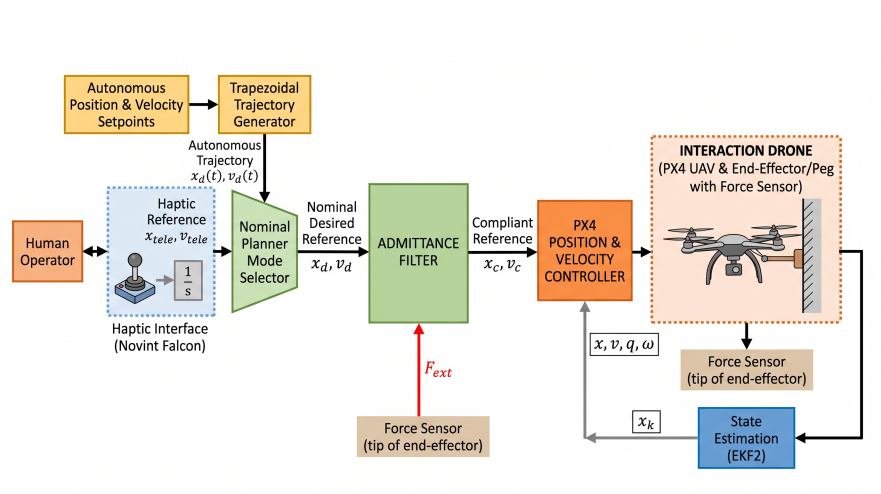
\includegraphics[width=\linewidth]{Immagini/Capitolo4/INTERACTION_DRONE_scheme.png}
    \caption{Planning and control scheme describing Interaction UAV architecture}
    \label{fig:placeholder}
\end{figure}
\subsection{High-Level Planner}
The high-level planner is responsible for generating a nominal Cartesian trajectory, denoted as $\mathbf{x}_d(t)$, which guides the inspection drone from its initial hovering state to the target surface. This reference trajectory dictates the desired 3D position and heading over time, ensuring a smooth and bounded approach velocity. However, this planned path is purely kinematic and geometric; it assumes a free-space environment and does not account for the reaction forces that arise upon impact. During the free-flight phase, the underlying flight controller tracks $\mathbf{x}_d(t)$ precisely. Yet, if the drone were to persistently track this rigid setpoint after establishing contact with the wall, the spring force by positional error action of the position controller united with integral action would rapidly accumulate error, leading to actuator saturation, violent rebounds, and inevitable instability.

\subsection{Admittance Filter}
To safely manage the transition and maintain a stable physical interaction, an admittance control strategy is implemented. This framework renders the drone compliant to external forces by masking the rigid structure as a virtual mass-spring-damper system. The core of the admittance filter~\cite{siciliano2008springer} is governed by the following second-order differential equation:
\begin{equation}
    \mathbf{M}_d \ddot{\mathbf{e}} + \mathbf{D}_d \dot{\mathbf{e}} + \mathbf{K}_d \mathbf{e} = \mathbf{F}_{ext}
\end{equation}
where $\mathbf{e}(t) = \mathbf{x}_c(t) - \mathbf{x}_d(t)$ represents the positional deviation between the newly generated compliant reference $\mathbf{x}_c(t)$ and the nominal planner trajectory $\mathbf{x}_d(t)$. The matrices $\mathbf{M}_d$, $\mathbf{D}_d$, and $\mathbf{K}_d$ are positive-definite diagonal matrices representing the desired virtual mass, damping, and stiffness, respectively. The vector $\mathbf{F}_{ext}$ represents the external contact force measured by the end-effector's onboard force sensor.
\\By numerically integrating this dynamic equation in real time, the filter evaluates the necessary spatial deviation and outputs the compliant setpoint $\mathbf{x}_c(t)$. The behavior of the system is thus completely shaped by the chosen virtual parameters. During free flight, since the measured external force is zero ($\mathbf{F}_{ext} = \mathbf{0}$), the positional error $\mathbf{e}(t)$ converges to zero, and the compliant reference matches the nominal one ($\mathbf{x}_c = \mathbf{x}_d$). Upon impact, the reaction force $\mathbf{F}_{ext}$ drives the admittance dynamics, causing the compliant reference to yield backward. This dynamically adjusted setpoint $\mathbf{x}_c(t)$ is continuously fed to the standard PX4 cascaded PID controller. As a result, the drone safely absorbs the impact and maintains a steady pressure against the surface, achieving the desired contact force without destabilizing the flight dynamics.

%%%%%%%%%%%%%%%%%%%%%%%% SHARED CONTROL %%%%%%%%%%%%%%%%%%%%%%%%%%%%%

\section{Human-Robot Shared Control}
\subsection{Teleoperation Modalities}
The proposed shared autonomy architecture allows the human operator to intervene in the mission through a haptic interface.
\begin{figure}[h!]
    \centering
    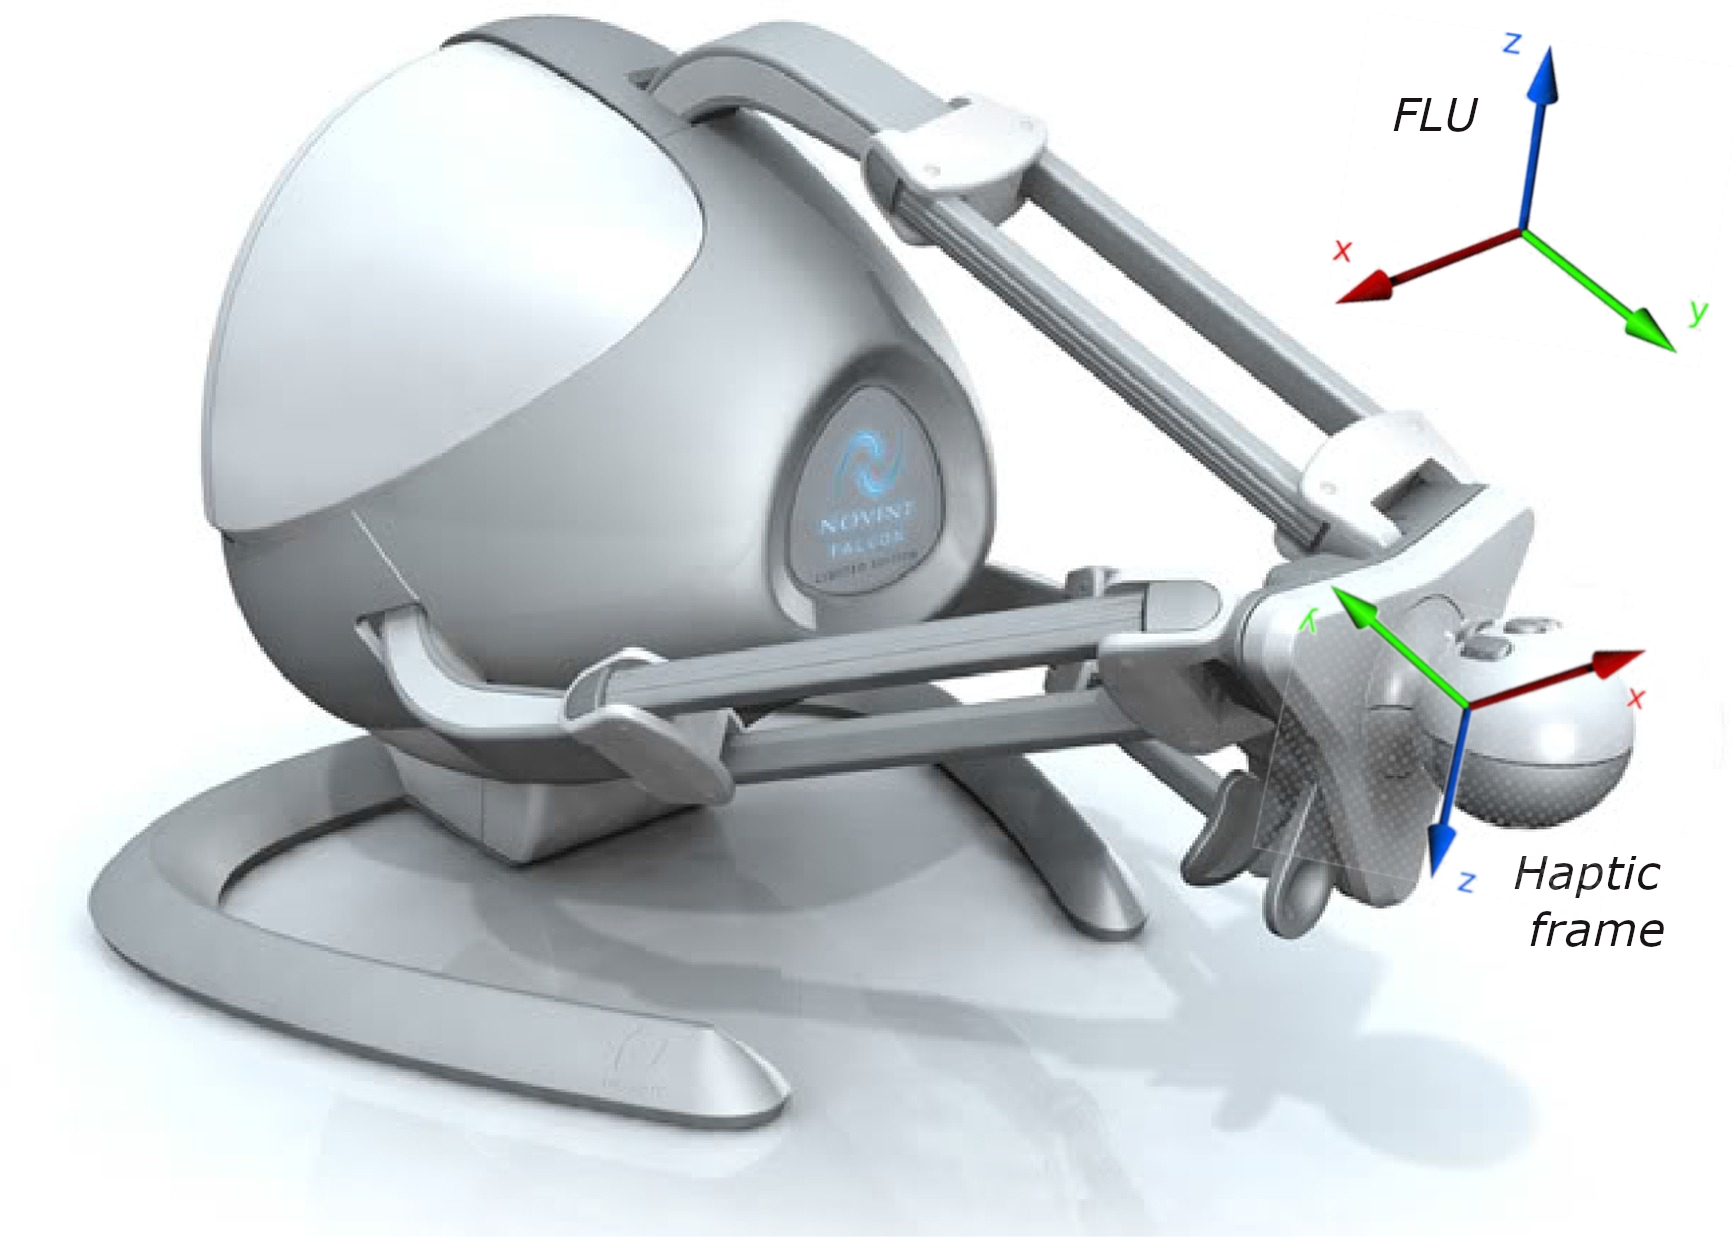
\includegraphics[width=0.5\linewidth]{Immagini/Capitolo4/Falcon_render.jpg}
    \caption{Haptic Interface Novint Falcon, used in simulations and experiments}
    \label{fig:placeholder}
\end{figure}
Depending on the operational phase and the specific mission requirements, the user can interact with the robotic team using two distinct teleoperation modalities:
\begin{itemize}
    \item \textbf{Observer Drone Control Mode:} The operator dynamically adjusts the Point of View of the camera drone. By manipulating the haptic device, the user modifies the relative distance, relative height, and azimuth angle around the inspection target. This mode enhances situational awareness and allows the operator to inspect specific structural details without disrupting the autonomous tracking.
    \item \textbf{Interaction Drone Control Mode:} During the critical phase of physical interaction, the operator can take direct control of the inspection drone to guide the fine insertion maneuver. In this phase, the human's cognitive judgment and dexterity are coupled with the autonomous admittance filter, which guarantees physical stability upon contact with the environment.
\end{itemize}

\subsection{Reference Generation via Haptic}
The used device, Novint Falcon, provides a physical 3D workspace of approximately $10 \times 10 \times 10$ cm, offering three translational degrees of freedom.  To mitigate the effects of sensor noise and unintentional operator tremors within this confined workspace, a nonlinear deadband with a threshold $d$ is applied to the raw input:
\begin{equation}
    f_{\text{db}}(x, d) = 
    \begin{cases} 
      0 & \text{if } |x| < d \\
      x - \operatorname{sgn}(x)d & \text{if } |x| \geq d
   \end{cases},
\end{equation}
\begin{figure}[h!]
    \centering
    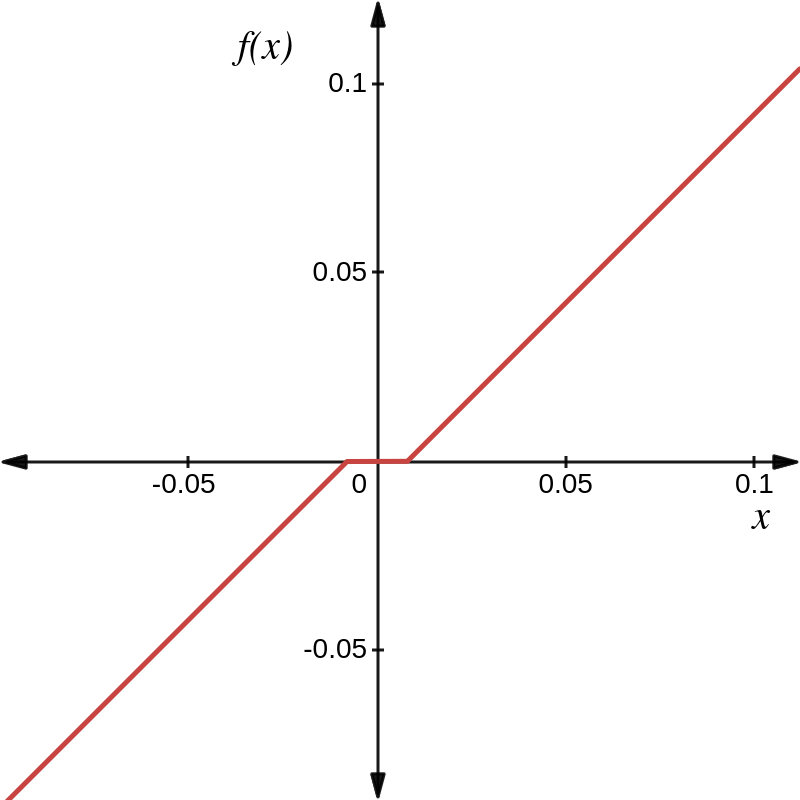
\includegraphics[width=0.5\linewidth]{Immagini/Capitolo4/Nonlinear_deadband_force.png}
    \caption{Nonlinear deadband applied on force given by the user on haptic device, $d=0.008$}
    \label{fig:haptic_render}
\end{figure}
where in this case $x\in[-0.1,0.1]$ m is a generic haptic end-effector coordinate in haptic frame (\ref{fig:haptic_render})(see Appendix \ref{app:implementation_details}). When operating in the observer control mode, the haptic interface is utilized to dynamically command the 3D reference for the camera drone in cylindrical coordinates[\ref{eq:cyl_mapping}]: this provides a human intuitive commanding modality for a target tracking, in relation to what he sees and which movements he can really perform with an underactuated drone (i.e, it would be useless to use spherical coordinates for 4 DOF UAV).  
In order to maintain consistency with the OCP formulation, the displacements of the haptic end-effector are directly mapped into reference velocities for the cylindrical variables. Specifically, the $x_h$, $y_h$, and $z_h$ inputs govern the rate of change of the radial distance $\dot{r}_{cyl}$, the azimuth orbit $\dot{\beta}$, and the relative altitude $\dot{z}_{rel}$, respectively. The position of device's end-effector in this operational space is denoted as $\mathbf{p}_h = [x_h, y_h, z_h]^\top$ and there is, clearly, the necessity to translate such small movements in bigger ones for feeding the drone with a proper reference. By introducing a generic scaling factor $K_{\text{joy}}=15$, the reference velocities imposed by the user are defined as:
\begin{equation}
    \begin{bmatrix} \dot{r}_{cyl} \\ \dot{\beta} \\ \dot{z}_{rel} \end{bmatrix} = 
    K_{\text{joy}} \begin{bmatrix} 
    v_{r,\max} \cdot f_{\text{db}}(x_h, d) \\ 
    v_{\beta,\max} \cdot f_{\text{db}}(y_h, d) \\ 
    v_{z,\max} \cdot f_{\text{db}}(z_h, d) 
    \end{bmatrix}
\end{equation}
These velocities are numerically integrated over the control loop time step $\Delta t$ to generate the desired cylindrical reference vector. To avoid kinematic singularities and physically unfeasible setpoints, bounds are applied during the integration step: the radial distance is strictly kept above a minimum safety threshold (avoiding singularity in $r=0$), and the azimuth angle is wrapped within the $[-\pi, \pi]$ interval to ensure continuity in rotation. The resulting updated reference vector $\mathbf{y}_{\text{ref}}(t) = [r_{cyl,\text{ref}}, \beta_{\text{ref}}, z_{rel,\text{ref}}]^\top$ is then published to the MPC planner, dynamically shifting the optimal tracking objective.

\subsection{Force Feedback Management}
\label{section:APF}
Force feedback has been handled with a sum of two contribution given back to the user.
\\A base mechanical impedance is applied to provide the user with a tactile sensation of stability and centering with respect to the origin (i.e., zero imposed velocity). This behavior is modeled as a virtual spring-damper system:
\begin{equation}
    \mathbf{F}_{\text{imp}} = -k \cdot \mathbf{p}_h - b \cdot \dot{\mathbf{p}}_h
\end{equation}
In addition to this base impedance, to ensure the safety of the visual tracking maneuver and prevent the observer drone from losing sight of the target or getting too close to it, a haptic force feedback based on Artificial Potential Fields is also rendered to the operator. This feedback translates undesired behaviors for the drone into a physical sensation for the human.
\\To do this, we need to mathematically define the physical boundaries of the camera's optical frustum and the drone's safety area. These boundaries impose spatial constraints that are continuously compared with the actual measured state $\mathbf{y}_{\text{act}} = [r_{\text{act}}, \beta_{\text{act}}, z_{\text{act}}, \psi_{\text{dev}}]^\top$, where $\psi_{\text{dev}}$ is the yaw deviation of the target from the camera's optical center.
\\First, let us define the vertical physical limit of the camera's vision. From a top-down perspective, if the target is at a radial distance $r_{\text{act}}$, its projected depth along the camera's optical axis is $r_{\text{act}} \cos(\psi_{\text{dev}})$. Using basic trigonometry on the vertical plane, the maximum visible height from the center of the image to the top or bottom edge is defined as:
\begin{equation}
    z_{\max} = r \cos(\psi_{\text{dev}}) \tan\left(\frac{\text{FOV}_v}{2}\right)
\end{equation}
\begin{figure}[htbp]
    \centering
    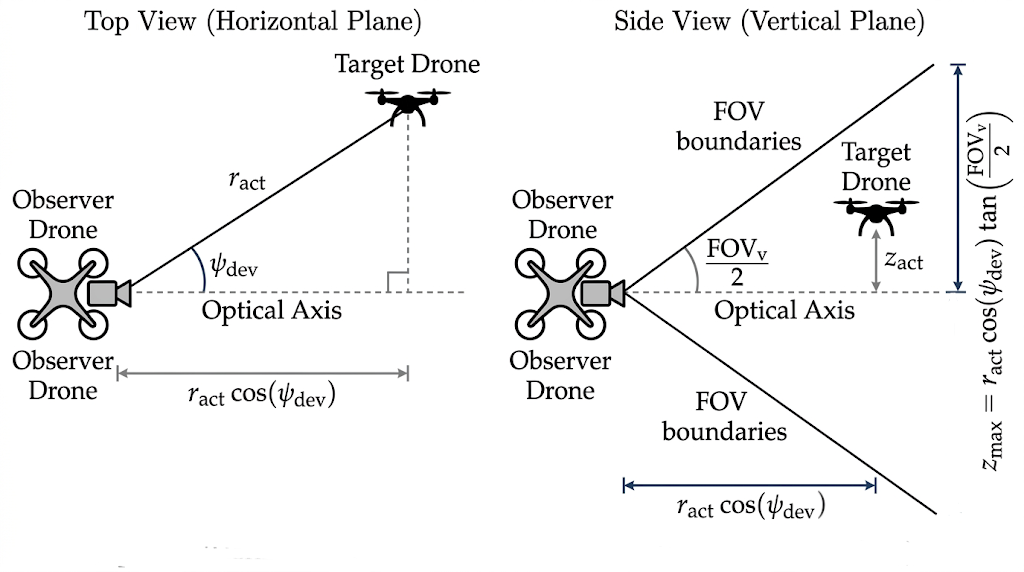
\includegraphics[width=\linewidth]{Immagini/Capitolo4/FOV_boundaries.png}
    \caption{Top and side views of the two drones}
    \label{fig:placeholder}
\end{figure}
\justify
where $FOV_v$ is a parameter denoting the maximum vertical optical aperture of the camera. 
\\\textbf{Notice}: this is an approximation. This supposes the camera optical axes to be always parallel to world XY plane (i.e., flat drone). Since camera is rigidly mounted on Observer Drone body frame, UAV must roll and pitch in order to move. This could be avoided by bringing distance in Observer UAV's body frame, but it's acceptable for smooth desired motion.
\\Using $z_{\max}$, we can easily define the distances from the actual drone state to the boundaries of the image. These spatial margins are geometrically defined as follows:
\begin{align}
    \Delta r &= r_{\text{act}} - r_{\min} \\
    \Delta z_{\text{top}} &= z_{\max} - z_{\text{act}} \\
    \Delta z_{\text{bot}} &= z_{\text{act}} + z_{\max} \\
    \Delta \psi &= \frac{\text{FOV}_h}{2} - |\psi_{\text{dev}}|
\end{align}
\begin{figure}[h!]
    \centering
    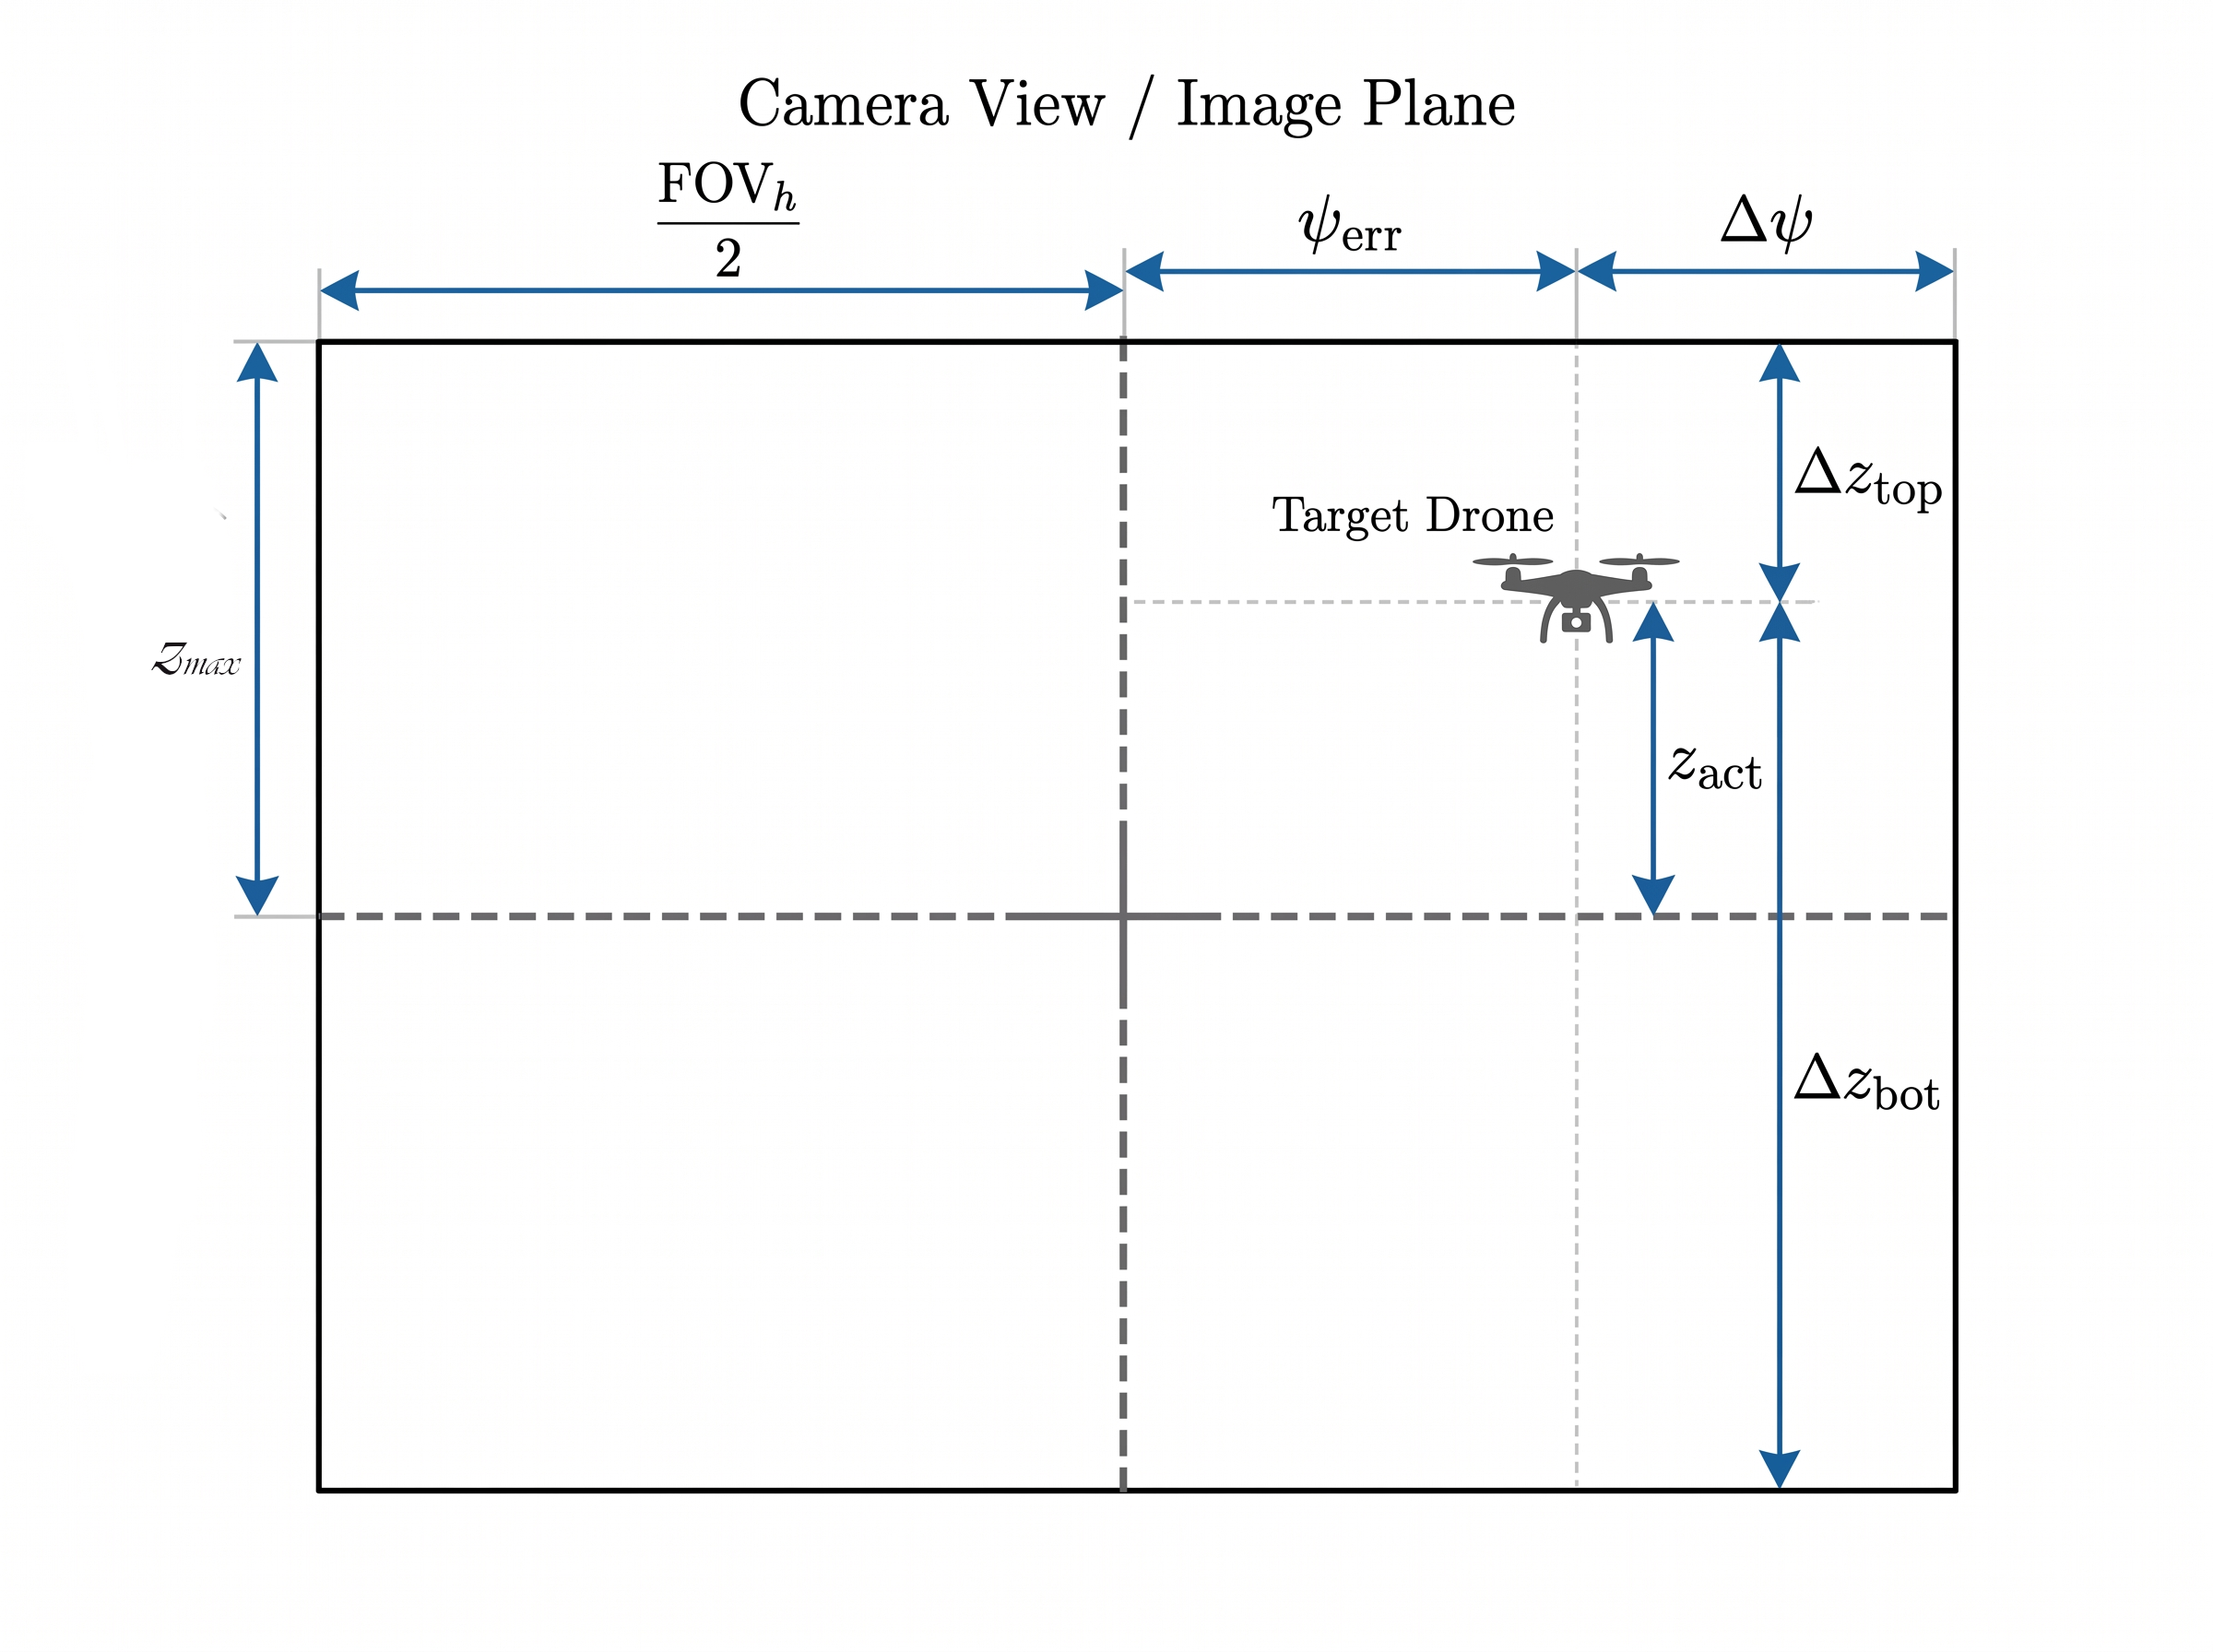
\includegraphics[width=0.8\linewidth]{Image_plane_boundaries.png}
    \caption{FOV boundaries in camera image plane}
    \label{fig:placeholder}
\end{figure}
where $r_{\min}$ ensures collision avoidance, the $z$ distances represent the remaining margins from the vertical limits of the Field of View ($\text{FOV}_v$), and $\Delta \psi$ represents the distance from the horizontal limits ($\text{FOV}_h$).
\\When any of these distances falls below a predefined activation threshold $d_{\text{act}}$, an exponential repulsive force is triggered. For a generic distance $d$, the intensity of the force is formulated as:
\begin{equation}
    \label{eq:repulsive_force}
    F_{\text{rep}}(d) = 
    \begin{cases} 
      0 & \text{if } d \geq d_{\text{act}} \\
      k_{\text{rep}} \left( e^{\left( \alpha \frac{d_{\text{act}} - d}{d_{\text{act}}} \right)} - 1 \right) & \text{if } 0 < d < d_{\text{act}} \\
      F_{\max}^{\text{rep}} & \text{if } d \leq 0
   \end{cases}
\end{equation}
where $\alpha$ is a tunable shaping factor that determines the exponential steepness of the virtual boundary, and $k_{\text{rep}}$ is the scaling gain. To satisfy the boundary condition, $k_{\text{rep}}$ is analytically derived from the maximum allowable torque $F_{\max}^{\text{rep}}$ as:
\begin{equation}
    k_{\text{rep}} = \frac{F_{\max}^{\text{rep}}}{e^\alpha - 1}
\end{equation}
In this way, the workspace is partitioned into three distinct operational regions:
\begin{itemize}
    \item \textbf{Free Region ($d \geq d_{\text{act}}$):} The vehicle is well within safe operational limits. The repulsive force is identically zero ($F_{\text{rep}} = 0$), and the operator feels only the standard centering spring-damper impedance.
    \item \textbf{Anticipatory Repulsive Buffer ($0 < d < d_{\text{act}}$):} The state enters the safety buffer. The repulsive force ramps up exponentially according to~\eqref{eq:repulsive_force}, acting as a virtual tactile barrier that warns the human pilot of the approaching boundary before any constraint violation occurs.
    \item \textbf{Violation Region ($d \leq 0$):} The boundary has been breached. The repulsive force saturates at its maximum value $F_{\max}^{\text{rep}}$ to vigorously push the operator away from danger.
\end{itemize}
The specific activation thresholds $d_{\text{act}}$ adopted in this work are configured as follows:
\begin{itemize}
    \item For the \textbf{radial distance}, $d_{\text{act}} = r_{\min} = 1.5\text{ m}$. Thus, the repulsive force activates as soon as the standoff distance drops below $r < r_{\min} + d_{\text{act}} = 3.0\text{ m}$, providing a $1.5\text{ m}$ wide progressive warning zone before reaching the minimum collision distance $r_{\min}$.
    \item For the \textbf{camera vertical FoV}, $d_{\text{act}} = 0.3 \cdot z_{\max}$. Consequently, the central $70\%$ of the image height represents a free visual zone ($F_z^{\text{rep}} = 0$), while tactile resistance activates only when the target enters the outer $30\%$ approaching the top or bottom image borders.
    \item For the \textbf{camera horizontal FoV}, $d_{\text{act}} = 0.3 \cdot (\text{FOV}_h / 2)$, applying lateral correction forces only when the yaw misalignment exceeds $70\%$ of the semi-aperture.
\end{itemize}
\begin{figure}[h!]
    \centering
    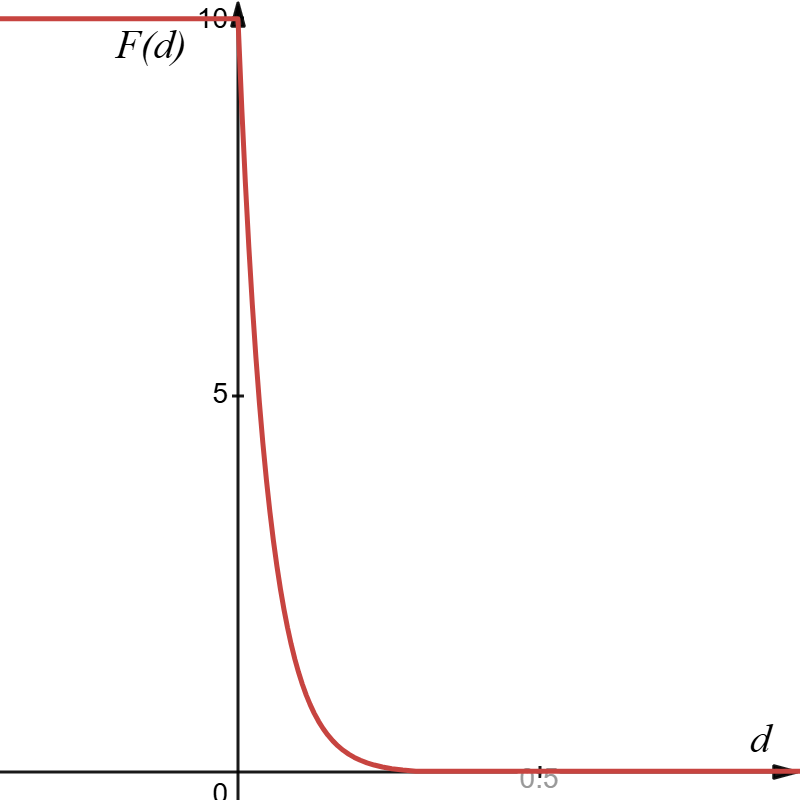
\includegraphics[width=0.6\linewidth]{Immagini/Capitolo4/F_rep.png}
    \caption{Repulsive force function $F_{rep}(d)$ - Repulsive force is maximum when $d=0$, decreases exponentially until becoming $F_{rep}=0$ N when $d\ge d_{act}$. Parameters: $\alpha=6$, $d_{act}=0.3$, $F_{max}=10$ N}
    \label{fig:placeholder}
\end{figure}
\\The   haptic interface axes $x, y$, and $z$ (defined in a standard Forward-Left-Up reference frame) directly govern the radial, azimuthal, and vertical velocity commands, respectively. Therefore, the computed scalar repulsive forces are mapped onto these corresponding operational axes to intuitively counteract unsafe human inputs:
\begin{equation}
\begin{aligned}
    F_{x}^{\text{rep}} &= F_{\text{rep}}(\Delta r) \\
    F_{y}^{\text{rep}} &= - \operatorname{sgn}(\psi_{\text{dev}}) \cdot F_{\text{rep}}(\Delta \psi) \\
    F_{z}^{\text{rep}} &= - F_{\text{rep}}(\Delta z_{\text{top}}) + F_{\text{rep}}(\Delta z_{\text{bot}})
\end{aligned}
\end{equation}
The horizontal feedback $F_{y}^{\text{rep}}$ acts directly on the yaw alignment error, pushing the operator's hand to correct tracking misalignment, while the radial and vertical forces prevent physical collisions and boundary violations.
The total force commanded to the motors of the haptic device is the superimposition of the base mechanical impedance and the visual repulsive fields, eventually saturated by the hardware limits ($F_{\max}$) to prevent mechanical damage:
\begin{equation}
    \mathbf{F}_{\text{tot}} = \operatorname{sat}\left( \mathbf{F}_{\text{imp}} + \mathbf{F}^{\text{rep}}, \pm F_{\max} \right)
\end{equation}
By combining these components, the operator naturally perceives the center of the workspace as a stable equilibrium, while the camera FOV limits and safety distances feel like elastic, repulsive walls that actively guide the teleoperation.